\chapter{Results and Discussion}

This chapter presents the major outputs of the study, including the construction of the Akeanon text and speech corpora, and the performance evaluation of the developed ASR model.
\section{Constructed Akeanon Text Corpus}
A total of \textbf{25,800} Akeanon words were collected and verified for the text corpus. This collection excludes the Swadesh and SIL word lists and includes a wide variety of root words, derivations, and inflections. Figure~\ref{fig:text-corpus} shows a snapshot of the sheet file that serves as the database of the text corpus.

\begin{figure}[H]
    \centering
    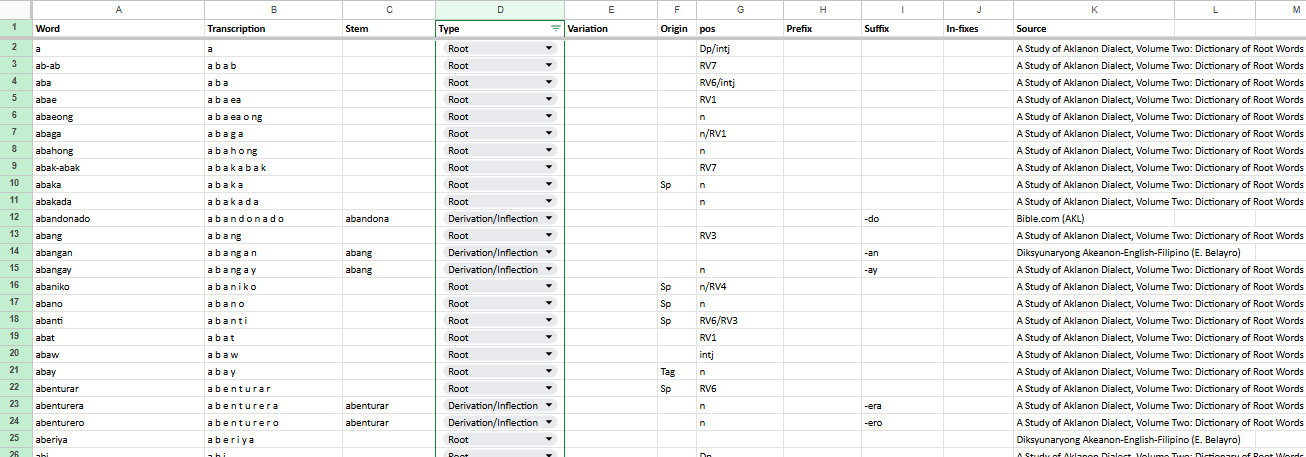
\includegraphics[width=\textwidth]{./figures/text-corpus.png}
    \caption{Snapshot of the Akeanon text corpus}
    \label{fig:text-corpus}
\end{figure}

In addition to the main corpus, the study also translated the Swadesh 207-word list and SIL International's word list into five Akeanon dialects: Common Akeanon, Bukidnon, Buruangganon, Malaynon, and Nabasnon. Figures~\ref{fig:swadesh-list} and~\ref{fig:sil-list} display sample entries from these translations.

\begin{figure}[H]
    \centering
    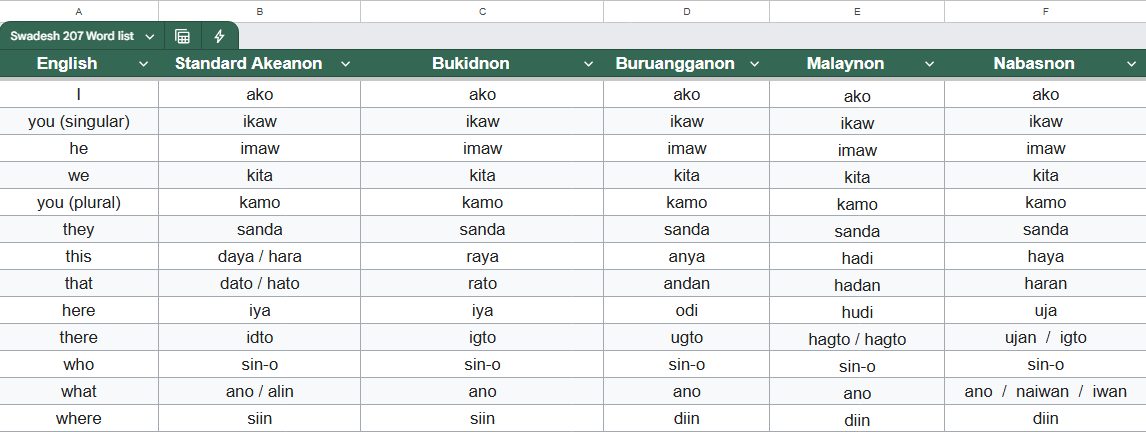
\includegraphics[width=\textwidth]{./figures/swadesh.png}
    \caption{Akeanon translations of the Swadesh 207-word list}
    \label{fig:swadesh-list}
\end{figure}

\begin{figure}[H]
    \centering
    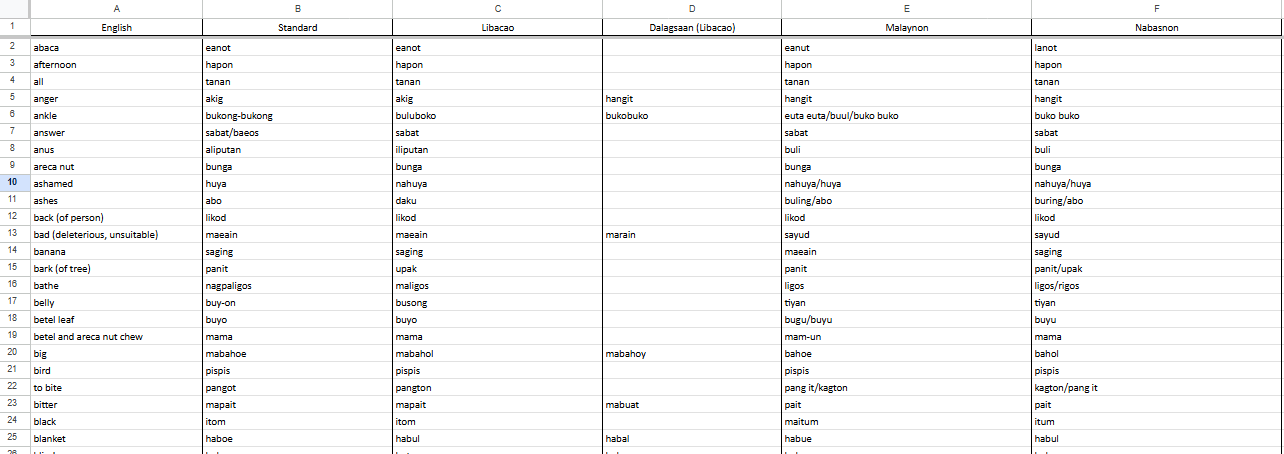
\includegraphics[width=\textwidth]{./figures/SIL.png}
    \caption{Akeanon translations of SIL International's word list}
    \label{fig:sil-list}
\end{figure}

The constructed text corpus serves as a foundation for the development of the Akeanon ASR system, providing linguistic diversity and coverage across different dialects.

\section{Constructed Akeanon Speech Corpus}

\subsection{Speech Data}
For the Akeanon speech corpus, \textbf{100} voice recordings were collected, equivalent to over \textbf{8 hours} of raw data, along with additional \textbf{31 hours} of extracted audio from online resources. Each recording corresponds to one of the generated text sets and covers various dialects and speaker demographics.

The collected speech data provides the necessary acoustic material for training, validating, and testing the ASR models. The recordings include natural variations in pronunciation, intonation, and pacing, enriching the acoustic modeling phase.

\begin{table}[H]
	\centering
	\begin{adjustbox}{width=0.95\textwidth}
		\begin{tabular}{lllcc}
			\toprule
			\textbf{CATEGORY} & \textbf{SUBCATEGORY} & \multicolumn{2}{c}{\textbf{GENDER}} & \textbf{AUDIO DURATION} \\
			\cmidrule(lr){3-4}
			& & \textbf{M} & \textbf{F} & \\
			\midrule
			\multicolumn{5}{l}{\textbf{Sets}} \\
			& Set A & 4 & 6 & 01:14:33 \\
			& Set B & 2 & 8 & 01:11:08 \\
			& Set C & 3 & 7 & 01:14:33 \\
			& Set D & 2 & 8 & 01:10:28 \\
			& Set E & 2 & 8 & 01:13:05 \\
			\addlinespace
			& \textbf{Total} & \textbf{13} & \textbf{37} & \textbf{06:03:47} \\
			\addlinespace
			\multicolumn{5}{l}{\textbf{Dialects}} \\
			& Common Akeanon & 2 & 8 & 00:30:46 \\
			& Libacao          & 3 & 7 & 00:30:00 \\
			& Nabasnon         & 4 & 6 & 00:27:25 \\
			& Malaynon         & 6 & 4 & 00:33:56 \\
			& Buruanganon      & 1 & 9 & 00:35:00 \\
			\addlinespace
			& \textbf{Total} & \textbf{16} & \textbf{34} & \textbf{02:37:07} \\
			\addlinespace
			\multicolumn{5}{l}{\textbf{Bible}} \\
			& — & 2 & 0 & 31:07:59 \\
			\addlinespace
			& \textbf{Total} & \textbf{2} & \textbf{0} & \textbf{31:07:59} \\
			\bottomrule
		\end{tabular}
	\end{adjustbox}
	\caption{Statistics for the constructed Akeanon speech corpus by sets, gender, and audio duration.}
	\label{tab:bikolano_stats}
\end{table}

\subsection{Phoneme Frequency Analysis}
A detailed phoneme frequency analysis was performed on the constructed speech corpus to better understand the distribution of sounds in Akeanon. This information is essential for optimizing acoustic modeling and ensuring that the ASR system is robust to the most common phonetic patterns.

Table~\ref{tab:phoneme-frequency} summarizes the frequency counts of each phoneme observed in the corpus. The five most frequent phonemes are \textit{a}, \textit{n}, \textit{i}, \textit{o}, and \textit{g}, which together account for a significant portion of the total phoneme occurrences. This distribution reflects the phonological characteristics of Akeanon and highlights the importance of accurately modeling these sounds.

\begin{table}[H]
	\centering
	\begin{tabular}{lc}
		\toprule
		\textbf{Phoneme} & \textbf{Frequency} \\
		\midrule
		a   & 5,112 \\
		n   & 1,671 \\
		i   & 1,606 \\
		o   & 1,542 \\
		g   & 1,217 \\
		u   & 1,073 \\
		t   & 1,069 \\
		m   & 984  \\
		k   & 936  \\
		p   & 877  \\
		s   & 822  \\
		b   & 738  \\
		d   & 598  \\
		l   & 591  \\
		ea  & 566  \\
		ng  & 500  \\
		h   & 493  \\
		y   & 437  \\
		r   & 369  \\
		w   & 295  \\
		e   & 172  \\
		sh  & 28   \\
		ch  & 16   \\
		dy  & 14   \\
		ts  & 4    \\
		v   & 2    \\
		z   & 1    \\
		\bottomrule
	\end{tabular}
	\caption{Phoneme frequency counts of the constructed Akeanon speech corpus.}
	\label{tab:phoneme-frequency}
\end{table}

The results of this analysis can guide future improvements in lexicon design, pronunciation modeling, and targeted data augmentation for underrepresented phonemes.

\section{Monophone and Triphone Model Results}

\subsection{Recognition Performance}

The recognition performance of the developed acoustic models was assessed using the Word Error Rate (WER), a standard metric that quantifies the proportion of incorrectly recognized words relative to the total number of words in the test set. Table~\ref{tab:wer-results} presents the WER achieved by each model configuration.

\begin{table}[H]
	\centering
	\renewcommand{\arraystretch}{1.3}
	\setlength{\tabcolsep}{16pt}
	\caption{Word Error Rate (WER\%) for Different Acoustic Models}
	\label{tab:wer-results}
	\begin{tabular}{|l|c|}
		\hline
		\textbf{Model} & \textbf{WER (\%)} \\
		\hline
		Monophone & 43.64 \\
		Triphone with Delta Features & 6.75 \\
		Triphone + LDA+MLLT & 5.49 \\
		SAT & 5.65 \\
		\hline
	\end{tabular}
\end{table}

The results demonstrate a substantial reduction in WER as model complexity increases. The basic monophone model produced the highest error rate, indicating limited modeling capacity for acoustic variability. Incorporating triphone modeling with delta features resulted in a dramatic improvement, while further enhancements using LDA+MLLT transformations yielded the lowest WER. The Speaker Adaptive Training (SAT) model also performed well, confirming the benefit of speaker normalization techniques. Overall, these findings highlight the importance of advanced acoustic modeling and feature transformation methods in improving ASR accuracy for Akeanon. Furthermore, the successful training and evaluation of these models demonstrate the training feasibility of the constructed text and speech corpus, validating its adequacy for ASR development.
